\documentclass[a4paper,twoside]{article}
\usepackage[T1]{fontenc}
\usepackage[bahasa]{babel}
\usepackage{graphicx}
\usepackage{graphics}
\usepackage{float}
\usepackage[cm]{fullpage}
\pagestyle{myheadings}
\usepackage{etoolbox}
\usepackage{setspace} 
\usepackage{lipsum} 
\setlength{\headsep}{30pt}
\usepackage[inner=2cm,outer=2.5cm,top=2.5cm,bottom=2cm]{geometry} %margin
% \pagestyle{empty}

\makeatletter
\renewcommand{\@maketitle} {\begin{center} {\LARGE \textbf{ \textsc{\@title}} \par} \bigskip {\large \textbf{\textsc{\@author}} }\end{center} }
\renewcommand{\thispagestyle}[1]{}
\markright{\textbf{\textsc{Laporan Perkembangan Pengerjaan Skripsi\textemdash Sem. Ganjil 2018/2019}}}

\onehalfspacing
 
\usepackage[plainpages=false,pdfpagelabels,unicode]{hyperref}
\usepackage{listings}
\usepackage[table]{xcolor}

\lstdefinelanguage{plaintext}{
  sensitive=false,
  comment=[l]{//},
  morecomment=[s]{/*}{*/},
  identifierstyle=\color{black},
  morestring=[b]',
  morestring=[b]"
}

\lstset
{ 
    language=plaintext,
    basicstyle=\footnotesize,
    numbers=left,
    stepnumber=1,
    showstringspaces=false,
    tabsize=1,
    breaklines=true,
    breakatwhitespace=false,
    frame=leftline
}
 
\begin{document}

\title{\@judultopik}
\author{\nama \textendash \@npm} 

%ISILAH DATA BERIKUT INI:
\newcommand{\nama}{Billy Adiwijaya}
\newcommand{\@npm}{2015730053}
\newcommand{\tanggal}{15/11/2018} %Tanggal pembuatan dokumen
\newcommand{\@judultopik}{PEMBANGKIT TIMELAPSE PENGEMBANGAN PROYEK
PERANGKAT LUNAK BERBASIS WEB} % Judul/topik anda
\newcommand{\kodetopik}{PAN4401}
\newcommand{\jumpemb}{1} % Jumlah pembimbing, 1 atau 2
\newcommand{\pembA}{Pascal Alfadian Nugroho} 
\newcommand{\pembB}{-}
\newcommand{\semesterPertama}{45 - Ganjil 18/19} % semester pertama kali topik diambil, angka 1 dimulai dari sem Ganjil 96/97
\newcommand{\lamaSkripsi}{1} % Jumlah semester untuk mengerjakan skripsi s.d. dokumen ini dibuat
\newcommand{\kulPertama}{Skripsi 1} % Kuliah dimana topik ini diambil pertama kali
\newcommand{\tipePR}{B} % tipe progress report :
% A : dokumen pendukung untuk pengambilan ke-2 di Skripsi 1
% B : dokumen untuk reviewer pada presentasi dan review Skripsi 1
% C : dokumen pendukung untuk pengambilan ke-2 di Skripsi 2

% Dokumen hasil template ini harus dicetak bolak-balik !!!!

\maketitle

\pagenumbering{arabic}



\section{Data Skripsi} %TIDAK PERLU MENGUBAH BAGIAN INI !!!
Pembimbing utama/tunggal: {\bf \pembA}\\
Pembimbing pendamping: {\bf \pembB}\\
Kode Topik : {\bf \kodetopik}\\
Topik ini sudah dikerjakan selama : {\bf \lamaSkripsi} semester\\
Pengambilan pertama kali topik ini pada : Semester {\bf \semesterPertama} \\
Pengambilan pertama kali topik ini di kuliah : {\bf \kulPertama} \\
Tipe Laporan : {\bf \tipePR} -
\ifdefstring{\tipePR}{A}{
			Dokumen pendukung untuk {\BF pengambilan ke-2 di Skripsi 1} }
		{
		\ifdefstring{\tipePR}{B} {
				Dokumen untuk reviewer pada presentasi dan {\bf review Skripsi 1}}
			{	Dokumen pendukung untuk {\bf pengambilan ke-2 di Skripsi 2}}
		}
		
\section{Latar Belakang}
Git merupakan perangkat lunak \textit{Version Control Systems}\cite{chacon2014pro}.\textit{Version control} adalah sistem yang merekam perubahan pada \textit{file} atau sekumpulan \textit{file} dari waktu ke waktu. Perubahan yang terjadi pada \textit{repository} dicatat oleh Git dalam bentuk histori \textit{commit}. Setiap \textit{commit} mengandung informasi mengenai perubahan yang terjadi pada \textit{repository}, waktu perubahan, dan orang yang melakukan perubahan. \textit{Database} pada \textit{git} tidak bersifat terpusat, melainkan terdistribusi. Setiap orang yang terlibat mempunyai \textit{database} lokal pada masing-masing komputer, sehingga pengelolaan perangkat lunak dapat dilakukan secara \textit{online} dan \textit{offline}.

JGit adalah \textit{library} Java murni yang mengimplementasikan Git \textit{version control systems}\cite{JGit}. JGit dikembangkan oleh Eclipse Foundation. JGit bersifat \textit{open source}. Dengan menggunakan JGit, fitur-fitur dalam Git dapat diakses melalui program Java. 

Selenium adalah seperangkat alat yang secara khusus digunakan untuk mengotomatisasi \textit{web browsers}\cite{Selenium}. Dengan menggunakan Selenium WebDriver, pengguna dapat memasukkan \textit{script} bahasa pemrograman tertentu untuk melakukan pengujian. Bahasa pemrograman yang didukung yaitu C\#, Java, Perl, PHP, Python, Ruby, dan JavaScript. Selenium WebDriver dapat melakukan pengujian pada \textit{browser} Google Chrome, Mozilla Firefox, Opera, Safari, dan Internet Explorer.  
  
Pada skripsi ini, akan dibuat sebuah perangkat lunak yang dapat menampilkan animasi timelapse dari pengembangan proyek perangkat lunak berbasis web. Perangkat lunak ini dibangun menggunakan bahasa Java. Perangkat lunak ini menggunakan tampilan terminal/konsol. Dalam pembuatan animasi timelapse, dibutuhkan perangkat lunak Selenium WebDriver dan JGit.


\section{Rumusan Masalah}
Rumusan masalah dari skripsi ini adalah sebagai berikut:
\begin{enumerate}
	\item Bagaimana cara membangkitkan animasi \textit{timelapse} pada pengembangan proyek perangkat lunak berbasis web?
	\item Bagaimana cara mengimplementasikan aplikasi untuk membangkitkan \textit{timelapse} pada pengembangan proyek perangkat lunak berbasis web?
\end{enumerate}


\section{Tujuan}
Tujuan dari skripsi ini adalah sebagai berikut:
\begin{enumerate}
	\item Mengetahui cara untuk membangkitkan animasi \textit{timelapse} pada pengembangan proyek perangkat lunak berbasis web.
	\item Mengetahui cara untuk mengimplementasikan aplikasi untuk membangkitkan \textit{timelapse} pada pengembangan proyek perangkat lunak berbasis web.
\end{enumerate}



\section{Detail Perkembangan Pengerjaan Skripsi}
Detail bagian pekerjaan skripsi sesuai dengan rencan kerja/laporan perkembangan terkahir :
	\begin{enumerate}
		\item \textbf{Melakukan studi literatur tentang Selenium WebDriver, Git, dan JGit.}\\
		{\bf Status :} Ada sejak rencana kerja skripsi. \\
		{\bf Hasil :} \\

\begin{itemize}
\item \textbf{Git}\\
\end{itemize}
Git merupakan perangkat lunak \textit{Version Control Systems}. Pada bagian ini, dijelaskan mengenai \textit{Version Control Systems}, cara kerja Git, Git \textit{checkout}, dan operasi-operasi dasar pada Git. Subbab ini mengacu pada \cite{chacon2014pro}.   

\textbf{Version Control Systems}\\
\textit{Version Control Systems} adalah sistem yang merekam perubahan pada \textit{file} atau sekumpulan \textit{file} dari waktu ke waktu.\textit{Version Control Systems} biasanya digunakan  untuk merekam file yang berisi \textit{source code program}, tetapi pada kenyataannya \textit{Version Control Systems} dapat merekam hampir semua jenis file dalam komputer. Terdapat tiga jenis \textit{Version Control Systems}, yaitu: \textit{Local Version Control Systems}, \textit{Centralized Version Control Systems}, dan \textit{Distributed Version Control Systems}.

\textbf{Local Version Control Systems}\\
Metode \textit{version-controlled} yang banyak digunakan orang adalah dengan cara menyalin sekumpulan \textit{file} ke direktori lain. Namun cara tersebut rentan terhadap \textit{error}.
Misalnya, terdapat direktori A dan B, pengguna ingin mengubah \textit{file} yang terdapat pada direktori B, tetapi pengguna lupa kalau dia sedang berada di direktori A, maka pengguna mengubah \textit{file} pada direktori yang salah. Untuk mengatasi masalah tersebut, \textit{programmer} mengembangkan \textit{Local Version Control Systems}. 

\begin{figure}[H]
	\centering
		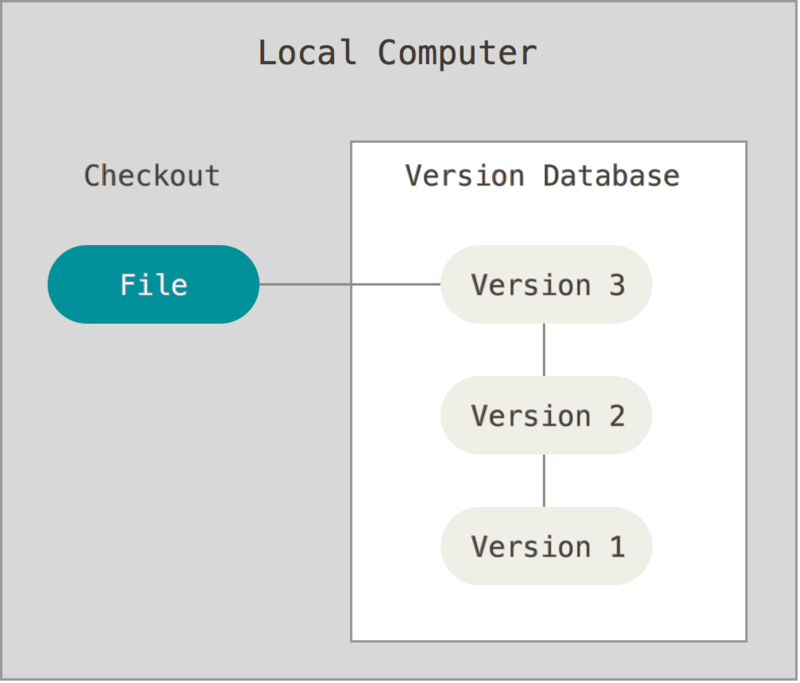
\includegraphics[scale=0.25]{Gambar/localvcs.png}
	\caption{Local version control\cite{chacon2014pro}.}
	\label{fig:localvcs}
\end{figure}

Gambar \ref{fig:localvcs} merupakan struktur dari \textit{Local Version Control Systems}. \textit{Database local Version Control Systems} ini tersimpan pada \textit{local directory} di komputer. \textit{Database} ini menyimpan perubahan \textit{file} ke dalam beberapa versi atau \textit{state}. \textit{Local Version Control}, dapat melakukan \textit{checkout} \textit{file} ke versi atau \textit{state} tertentu.   
 
\textbf{Centralized Version Control Systems}\\
\begin{figure}[H]
	\centering
		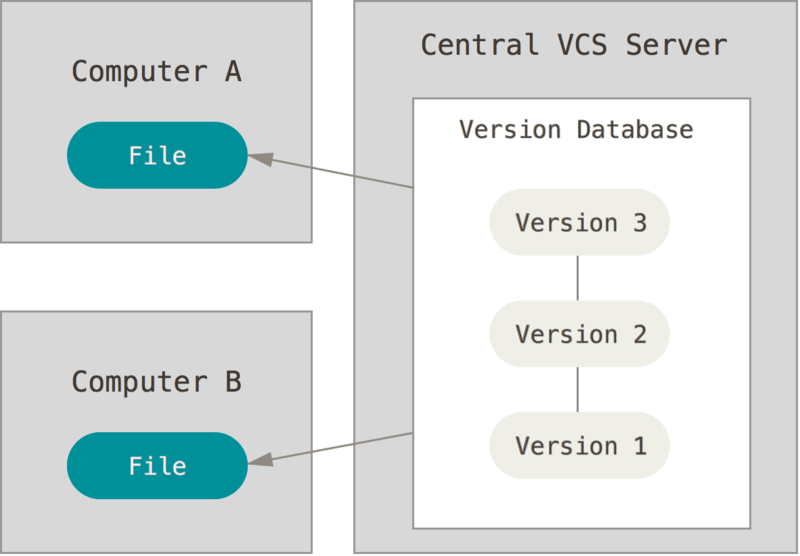
\includegraphics[scale=0.25]{Gambar/centralizedvcs.png}
	\caption{Centralized version control\cite{chacon2014pro}.}
	\label{fig:cvcs}
\end{figure}

\textit{Local Version Control} hanya menyimpan \textit{file} pada satu komputer saja. Muncul masalah baru ketika \textit{user} ingin berkolaborasi dengan \textit{user} lain. Untuk mengatasi masalah ini dikembangkan \textit{Centralized version control}. Gambar \ref{fig:cvcs} merupakan struktur dari \textit{Centralized Version Control Systems}. Dalam \textit{Centralized Control Version Systems} terdapat sebuah \textit{server} yang menyimpan setiap versi \textit{file}, dan klien yang dapat melakukan \textit{checkout} \textit{file}.

Sistem \textit{Centralized Version Control Systems} memiliki beberapa kelebihan. Setiap \textit{user}  dapat mengetahui pekerjaan yang dilakukan oleh \textit{user} lain. Administrator dapat lebih mudah mengontrol \textit{database} \textit{Centralized Version Control Systems} dibandingkan dengan \textit{database} \textit{Local Version Control Systems} dari setiap klien.      

Sistem \textit{Centralized Version Control Systems} memiliki kelemahan. Jika \textit{server} pusat \textit{Centralized Version Control Systems} mati , maka perubahan pada \textit{file} tidak bisa disimpan. Klien juga tidak dapat melakukan kolaborasi dengan klien lain. Jika \textit{harddisk} pada server rusak, maka semua versi \textit{file} akan hilang.  

\textbf{Distributed Version Control Systems}\\
\begin{figure}[H]
	\centering
		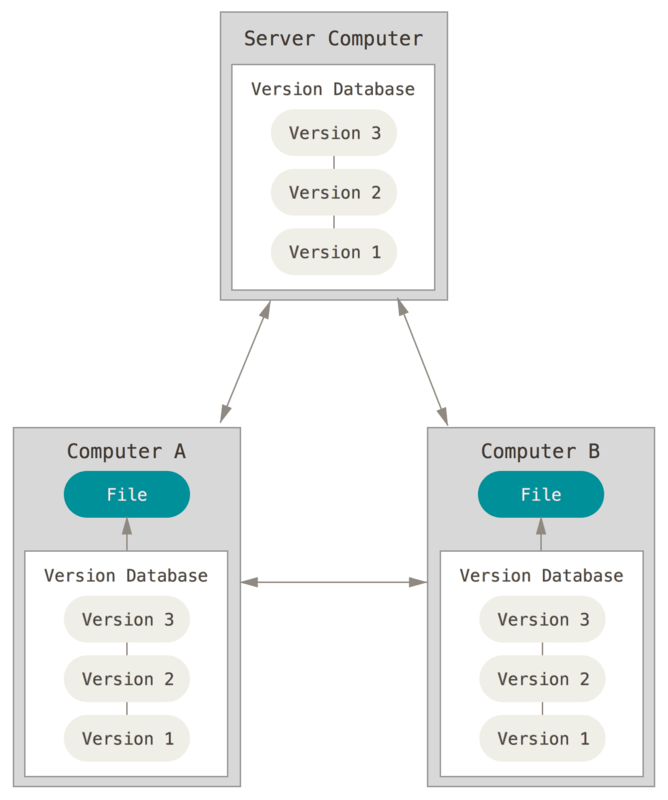
\includegraphics[scale=0.5]{Gambar/dvcs.png}
	\caption{Distributed version control\cite{chacon2014pro}.}
	\label{fig:dvcs}
\end{figure}
Gambar \ref{fig:dvcs} merupakan struktur dari \textit{Distributed Version Control Systems}. Dalam sebuah DVCS (seperti Git, Mercurial, Bazaar atau Darcs), klien tidak hanya melakukan \textit{checkout} untuk \textit{snapshot} terakhir setiap \textit{file}, namun klien juga memiliki salinan dari repositori tersebut. Dengan kata lain setiap klien memiliki \textit{version database local} pada komputernya. Jika server pusat mati, klien masih bisa melakukan kolaborasi dan klien manapun dapat mengirimkan kembali salinan repositori ke \textit{server}.

\textbf{Cara Kerja Git}\\
Salah satu perbedaan antara Git dengan VCS lainnya adalah dalam cara Git memperlakukan datanya. Kebanyakan sistem \textit{Version Control Systems} lain menyimpan informasi sebagai daftar perubahan \textit{file}. Pada Gambar \ref{fig:deltas}, terdapat tiga \textit{file}.\textit{Version Control Systems} menyimpan \textit{file} A, B, dan C pada versi pertama saja. Untuk versi kedua dan seterusnya yang disimpan adalah perubahan pada setiap \textit{file}. Sistem ini disebut juga sebagai \textit{delta-based Version Control Systems}. 
\begin{figure}[H]
	\centering
		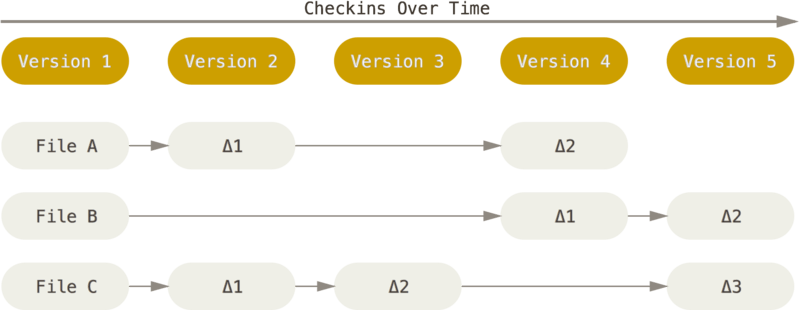
\includegraphics[scale=0.5]{Gambar/deltas.png}
	\caption{Menyimpan data sebagai \textit{snapshots} dari \textit{project}\cite{chacon2014pro}.}
	\label{fig:deltas}
\end{figure}


Berbeda dengan \textit{Version Control Systems} lainnya, Git memperlakukan datanya sebagai sebuah kumpulan \textit{snapshot} dari sebuah miniatur \textit{file system}. Setiap kali dilakukan \textit{commit}, git merekam \textit{state} dari sekumpulan \textit{file} dan menyimpanannya sebagai \textit{reference} \textit{snapshot} tersebut. Gambar \ref{fig:snapshots}, menunjukkan \textit{snapshots} dari \textit{file} A, B, dan C. Pada versi kedua, \textit{file} B tidak mengalami perubahan, sehingga \textit{file} yang disimpan adalah referensi \textit{file} B pada versi sebelumnya.
\begin{figure}[H]
	\centering
		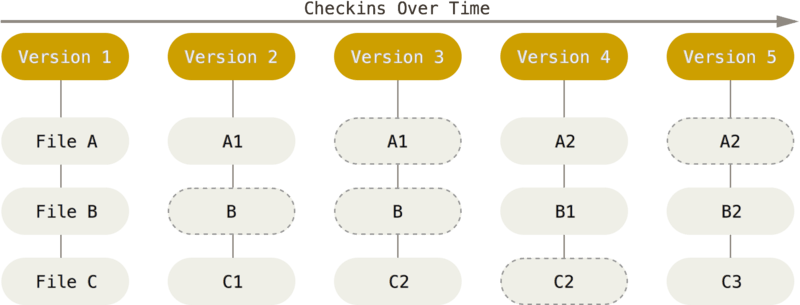
\includegraphics[scale=0.5]{Gambar/snapshots.png}
	\caption{Menyimpan data sebagai perubahan terhadap versi dasar dari setiap \textit{file}\cite{chacon2014pro}.}
	\label{fig:snapshots}
\end{figure}

\textbf{State pada Git}\\
Terdapat tiga \textit{state} pada Git yaitu \textit{committed}, \textit{modified}, and \textit{staged}.\textit{Committed} adalah \textit{state} dimana data sudah disimpan di \textit{local database}. \textit{Modified} \textit{state} dimana terdapat perubahan pada \textit{file}, namun \textit{file} tersebut belum di \textit{commit} ke \textit{database}. \textit{Staged} adalah \textit{state} dimana \textit{file} telah ditandai untuk kemudian dilakukan commit.

Terdapat tiga bagian utama dari sebuah \textit{project} Git yaitu direktori Git, \textit{working directory}, dan \textit{staging area}. Direktori Git merupakan tempat dimana Git menyimpan \textit{metadata} dan \textit{object database} dari \textit{project}. \textit{Working tree} adalah suatu \textit{snapshot} dari \textit{project}. Sekumpulan \textit{file} ini diambil dari \textit{database} di direktori Git dan ditempatkan pada \textit{disk} untuk digunakan dan dimodifikasi. \textit{Staging} area adalah \textit{file} yang menyimpan informasi mengenai apa yang menjadi \textit{commit} selanjutnya. \textit{File staging area} terdapat pada direktori Git. Untuk lebih jelasnya, lihat Gambar \ref{fig:git_state}.

Alur kerja dari Git adalah sebagai berikut:
\begin{enumerate}
\item Melakukan modifikasi pada \textit{file}.
\item Menandai perubahan pada \textit{file} dan memindahkannya ke \textit{staging area}.
\item Mengambil \textit{file} dari \textit{staging area} dan menyimpan \textit{snapshot} ke direktori Git. Proses ini disebut dengan \textit{commit}.
\end{enumerate}  

\begin{figure}[H]
	\centering
		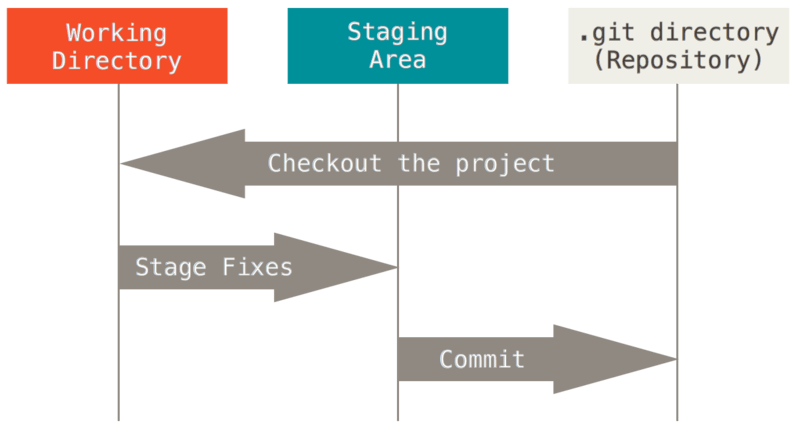
\includegraphics[scale=0.5]{Gambar/git_state.png}
	\caption{ \textit{Working tree}, \textit{Staging area}, dan Git direktori\cite{chacon2014pro}.}
	\label{fig:git_state}
\end{figure}

\textbf{Commit}\\
Commit merupakan sebuah \textit{snapshot} dari suatu \textit{file} atau direktori. \textit{Commit} menggambarkan \textit{state} dari \textit{working directory}. Gambar \ref{fig:snapshots} menunjukkan terdapat tiga \textit{file} pada versi/\textit{commit} keempat. Dimana terdapat \textit{file} A1, B1, dan C1 pada \textit{working directory}. \textit{File} A1, B1, dan C2  merupakan \textit{state} \textit{file} A, B, dan C pada \textit{commit} keempat. 

Git melakukan \textit{check-summed} pada \textit{commit} sebelum menyimpannya ke Git repositori. Mekanisme yang digunakan untuk melakukan \textit{check-summed} disebut dengan \textit{SHA-1 hash}. \textit{SHA-1 hash} terdiri dari empat puluh karakter heksadesimal(0-9 a-f). Nilai dari \textit{SHA-1 hash} dihitung berdasarkan isi dari \textit{working directory} atau struktur direktori Git.


\begin{lstlisting}[caption={Contoh histori commit dalam pengembangan perangkat lunak},label={lst:git_histori},language=plaintext]
C:\Users\user\Documents\GitHub\train-tracker-ellena-angelica>git log

commit b8aeacbd4743619b7b2d790d45bde26b899641e0 (HEAD -> master, origin/master, origin/HEAD)
Author: adamadamadamadamadam <adamnurmishwari@gmail.com>
Date:   Thu May 3 01:15:31 2018 +0700

    commitan terakhir. mastiin g buang memory sm batre

commit f836cc65bf6d50e274df54aa06c6fb529667aa06
Author: Evelyn Wijaya <evelynwijaya777@gmail.com>
Date:   Wed May 2 22:03:25 2018 +0700

    Update README.md

commit 2e1ce9a03a1f417326c3c6586503303cf6daf6b8
Author: Evelyn Wijaya <evelynwijaya777@gmail.com>
Date:   Wed May 2 22:01:10 2018 +0700

    Create README.md

commit 2f04488f9008745e8e6f67da33ffb2f6c2c9e747
Author: Evelyn Wijaya <evelynwijaya777@gmail.com>
Date:   Wed May 2 14:08:02 2018 +0700

    fix stasiun double

commit 7d8b66a9c6500de2753cdeac1084dc049c0c9f20
Author: Evelyn Wijaya <evelynwijaya777@gmail.com>
Date:   Wed May 2 13:32:21 2018 +0700

    fix stasiun double
    
\end{lstlisting}

Seperti yang diperlihatkan pada Listing \ref{lst:git_histori}, setiap \textit{commit} memiliki beberapa informasi. Baris pertama menunjukkan \textit{commit} ID yang berupa \textit{SHA-1 hash}. Pada baris ini, \textit{Master} menunjukkan \textit{branch} yang sedang aktif, \textit{master} juga merupakan \textit{pointer} ke \textit{commit} terakhir. \textit{Head} merupakan \textit{reference} ke \textit{branch master}. \textit{Origin}/\textit{master} dan \textit{origin}/\textit{HEAD} merupakan \textit{master} dan \textit{HEAD} pada \textit{remote repository}. Baris kedua menunjukkan orang yang melakukan \textit{commit} dan alamat emailnya. Baris ketiga menunjukkan waktu terjadinya \textit{commit}. Baris terakhir berisi deskripsi dari \textit{commit} tersebut.

\textbf{Operasi Dasar pada Git}\\
Pada bagian ini dijelaskan mengenai operasi dasar dalam Git dan sintaks-sintaksnya. Sintaks-sintaksnya ini dimasukkan pada Git \textit{command line}. Berikut ini adalah operasi-operasi dasar dalam Git:
\begin{enumerate}
\item Init\\
Operasi ini digunakan untuk membuat repositori lokal baru dengan nama tertentu. Bisa juga digunakan untuk merekam direktori yang sudah ada. Berikut adalah sintaks untuk melakukan operasi  \textit{init}:\\
\texttt{\$ git init [project-name]}  
\item Add\\
Operasi ini digunakan untuk menandai perubahan pada \textit{file} dan memindahkan \textit{file} tersebut ke \textit{staging area}. Operasi ini juga digunakan untuk menambahkan \textit{file} yang dipantau perubahannya. Berikut adalah sintaks untuk melakukan operasi add:\\
\texttt{\$ git add [file]}  
\item Commit\\
Operasi ini digunakan untuk merekam \textit{snapshot} atau \textit{state} \textit{file} atau sekumpulan \textit{file}. Operasi ini juga digunakan untuk memindahkan \textit{file} yang berada di \textit{stagging area} ke repositori Git. Berikut adalah sintaks untuk melakukan operasi \textit{commit}:\\
\texttt{\$ git commit -m "[descriptive message]"}  
\item Branch\\
Operasi ini digunakan untuk menampilkan semua \textit{branch} yang ada pada repositori Git, membuat \textit{branch} baru, dan menghapus \textit{branch}. Berikut adalah sintaks-sintaks untuk melakukan operasi \textit{branch}:\\
\texttt{\$ git branch}\\ 
\texttt{\$ git branch [branch-name]}\\
\texttt{\$ git branch -d [branch-name]}\\
\texttt{\$ git branch -D [branch-name]} 
\item Diff\\
Operasi ini digunakan untuk menampilkan perbedaan pada \textit{file} yang belum masuk \textit{staging area}, menampilkan perbedaan pada \textit{file} yang berada di \textit{staging area} dengan \textit{file} di \textit{commit} sebelumnya, dan perbedaan \textit{file} antara dua \textit{branch}.  Berikut adalah sintaks-sintaks untuk melakukan operasi \textit{diff}:\\
\texttt{\$ git diff} \\
\texttt{\$ git diff --staged}\\
\texttt{\$ git diff [first-branch]...[second-branch]}
\item Clone\\
Operasi ini digunakan untuk menyalin repositori Git yang berada di komputer lain atau suatu \textit{server}. Berikut adalah sintaks untuk melakukan operasi \textit{clone}:\\
\texttt{\$ git clone [url]}
\item Fetch\\
Operasi ini digunakan untuk mengambil data dari \textit{remote} repositori ke repositori lokal. Berikut adalah sintaks untuk melakukan operasi \textit{fetch}:\\
\texttt{\$ git fetch [bookmark]}
\item Merge\\
Operasi ini digunakan untuk menggabungkan \textit{branch} tertentu dengan \textit{branch} yang sedang aktif. Operasi ini juga digunakan untuk menggabungkan data yang diambil dari \textit{remote} repositori dengan data pada \textit{working directory}. Berikut adalah sintaks untuk melakukan operasi \textit{merge}:\\
\texttt{\$ git merge [branch]/[bookmark]}
\item Pull\\
Operasi ini adalah gabungan dari operasi \textit{fetch} dan \textit{merge}. Berikut adalah sintaks untuk melakukan operasi \textit{pull}:\\
\texttt{\$ git pull}
\item Push\\
Operasi ini digunakan untuk mengirim data pada reposipori Git lokal ke \textit{remote repository}.
Berikut adalah sintaks untuk melakukan operasi \textit{push}:\\
\texttt{\$ git push [alias] [branch]}
\item Checkout\\
Operasi ini digunakan untuk berpindah ke \textit{branch} atau \textit{commit} tertentu, setelah itu memperbarui \textit{file} pada \textit{working directory} berdasarkan \textit{branch} atau \textit{commit} tersebut. Berikut ini adalah sintaks-sintaks untuk operasi \textit{checkout}:\\
\texttt{\$ git checkout [SHA-1 commit]}\\
\texttt{\$ git checkout [branch-name]}
\item Log\\
Operasi ini digunakan untuk menampilkan semua histori \textit{commit} pada \textit{branch} yang sedang aktif. Berikut ini adalah sintaks untuk melakukan operasi \textit{log}:\\
\texttt{\$ git log}
\end{enumerate}

\textbf{Git Checkout}\\
Seperti yang sudah dijelaskan pada bagian Operasi Dasar Git, \textit{checkout} dapat digunakan untuk berpindah ke \textit{branch} atau \textit{commit} tertentu. Operasi \textit{checkout} dapat dilakukan menggunakan sintaks \texttt{\$ git checkout} diikuti dengan nama \textit{branch} atau \textit{SHA-1 hash}. Gambar \ref{fig:git_checkout} menunjukkan contoh \textit{checkout} pada \textit{commit}. Posisi awal \textit{HEAD} menunjuk pada \textit{branch master}, setelah dilakukan \textit{checkout} ke \textit{commit kedua}, posisi \textit{HEAD} menunjuk pada \textit{commit kedua}. \textit{Working directory} diperbarui berdasarkan \textit{state} pada \textit{commit} kedua. 

\textit{HEAD} yang menunjuk langsung ke suatu \textit{commit} disebut dengan \textit{detached HEAD}. Perubahan yang terjadi pada \textit{detached HEAD} tidak akan terekam oleh Git. Jika terdapat perubahan, kemudian dilakukan \textit{checkout commit} atau \textit{branch}, perubahan tersebut akan hilang. Tetapi, perubahan tersebut bisa disimpan dengan cara membuat \textit{branch} baru. Posisi \textit{HEAD} akan menunjuk pada \textit{branch} baru dan \textit{HEAD} sudah tidak lagi dalam keadaan \textit{detached HEAD}. 
\begin{figure}[H]
	\centering
		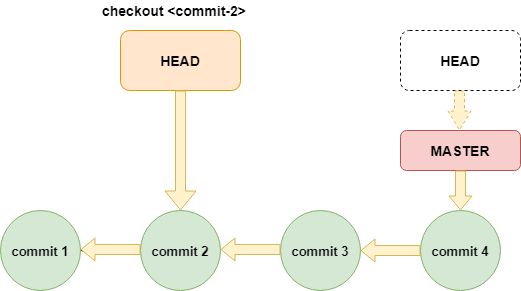
\includegraphics[scale=0.6]{Gambar/gitcheckoutcommit.png}
	\caption{\textit{Checkout} pada \textit{commit}}
	\label{fig:git_checkout}
\end{figure}

\begin{itemize}
\item \textbf{JGit}\\
\end{itemize}
JGit adalah \textit{library} Java murni yang mengimplementasikan Git \textit{version control systems}\cite{JGit}. Dengan menggunakan JGit, operasi-operasi dalam Git bisa dilakukan melalui program Java. Pada bagian ini dijelaskan beberapa kelas dari \textit{library} JGit. Subbab ini mengacu pada \cite{JGit_java_doc}. 

\textbf{Repository}\\
Kelas ini merepresentasikan repositori Git. Berikut ini adalah beberapa \textit{method} dalam kelas ini:
\begin{itemize}
\item public void create() throws IOException\\
Berfungsi untuk membuat repositori Git baru.
\item public void create(boolean bare) throws IOException\\
Berfungsi untuk membuat repositori Git baru. \\
Parameter: jika bernilai \textit{true} maka dibuat \textit{bare repository} (repositori tanpa \textit{working directory}). 
\item public String getBranch() throws IOException\\
Berfungsi untuk mendapatkan nama \textit{branch} yang ditunjuk oleh \textit{HEAD}, \textit{method} ini melempar \textit{IOException}.\\ 
Kembalian: nama dari \textit{branch} yang sedang aktif, contohnya \textit{master}.

\item public ObjectId resolve(String revstr) throws AmbiguousObjectException, IncorrectObjectTypeException, RevisionSyntaxException, IOException\\
Parameter: \textit{expression} dari \textit{git object references}. \textit{Method} ini melempar \textit{AmbiguousObjectException}, \textit{IncorrectObjectTypeException}, \textit{RevisionSyntaxException}, dan \textit{IOException}.\\
Kembalian: sebuah objek \textit{ObjectId}.
\end{itemize} 

\textbf{FileRepository}
Kelas ini merupakan turunan dari kelas \textit{Repository}. Berikut ini adalah \textit{construtor} dari kelas ini:
\begin{itemize}
\item public FileRepository(String gitDir) throws IOException\\
\textit{Constructor} ini membuat repositori berdasarkan parameter, \textit{constructor} ini melempar IOException.\\
Parameter: lokasi dari \textit{repository metadata}, lokasi ini berupa \textit{path}.
\end{itemize}

\textbf{Git}\\
Kelas ini menyediakan API yang mirip Git \textit{Command Line} untuk berinteraksi dengan repositori git. Berikut ini adalah \textit{constructor} dan beberapa \textit{method} dalam kelas ini:
\begin{itemize}
\item public Git(Repository repo)\\
\textit{Constructor} ini membuat objek Git yang digunakan untuk berinteraksi dengan repositori Git.
Parameter: objek \textit{Repository} yang digunakan untuk berinteraksi. Parameter tidak boleh bernilai \textit{null}. 

\item public static InitCommand init()\\
\textit{Method} ini mengembalikan objek \textit{command} untuk mengeksekusi operasi \textit{init}.\\
Kembalian: objek \textit{InitCommand} yang berfungsi untuk mengumpulkan parameter opsional dan akhirnya mengeksekusi operasi \textit{init}.

\item public AddCommand add()\\
\textit{Method} ini mengembalikan objek \textit{command} untuk mengeksekusi operasi \textit{add}.\\
Kembalian: objek \textit{AddCommand} yang berfungsi untuk mengumpulkan parameter opsional dan akhirnya mengeksekusi operasi \textit{add}.

\item public LogCommand log()\\
\textit{Method} ini mengembalikan objek \textit{command} untuk mengeksekusi operasi \textit{log}.\\
Kembalian: objek \textit{LogCommand} yang berfungsi untuk mengumpulkan parameter opsional dan akhirnya mengeksekusi operasi \textit{log}.

\item public CheckoutCommand checkout()\\
\textit{Method} ini mengembalikan objek \textit{command} untuk mengeksekusi operasi \textit{checkout}.\\
Kembalian: objek \textit{CheckoutCommand} yang berfungsi untuk mengumpulkan parameter opsional dan akhirnya mengeksekusi operasi \textit{checkout}.

\item public CommitCommand commit()\\
\textit{Method} ini mengembalikan objek \textit{command} untuk mengeksekusi operasi \textit{commit}.\\
Kembalian: objek \textit{CommitCommand} yang berfungsi untuk mengumpulkan parameter opsional dan akhirnya mengeksekusi operasi \textit{commit}.

\item public FetchCommand fetch()\\
\textit{Method} ini mengembalikan objek \textit{command} untuk mengeksekusi operasi \textit{fetch}.\\
Kembalian: objek \textit{FetchCommand} yang berfungsi untuk mengumpulkan parameter opsional dan akhirnya mengeksekusi operasi \textit{fetch}.

\item public PushCommand push()\\
\textit{Method} ini mengembalikan objek \textit{command} untuk mengeksekusi operasi \textit{push}.\\
Kembalian: objek \textit{PushCommand} yang berfungsi untuk mengumpulkan parameter opsional dan akhirnya mengeksekusi operasi \textit{push}.

\item public DiffCommand diff()\\
\textit{Method} ini mengembalikan objek \textit{command} untuk mengeksekusi operasi \textit{diff}.\\
Kembalian: objek \textit{DiffCommand} yang berfungsi untuk mengumpulkan parameter opsional dan akhirnya mengeksekusi operasi \textit{diff}.

\item public static CloneCommand cloneRepository()\\
\textit{Method} ini mengembalikan objek \textit{command} untuk mengeksekusi operasi \textit{clone}.\\
Kembalian: objek \textit{DiffCommand} yang berfungsi untuk mengumpulkan parameter opsional dan akhirnya mengeksekusi operasi \textit{clone}.

\item public MergeCommand merge()\\
\textit{Method} ini mengembalikan objek \textit{command} untuk mengeksekusi operasi \textit{merge}.\\
Kembalian: objek \textit{MergeCommand} yang berfungsi untuk mengumpulkan parameter opsional dan akhirnya mengeksekusi operasi \textit{merge}.

\item public PullCommand pull()\\
\textit{Method} ini mengembalikan objek \textit{command} untuk mengeksekusi operasi \textit{pull}.\\
Kembalian: objek \textit{PullCommand}.

\item public CreateBranchCommand branchCreate()\\
\textit{Method} ini mengembalikan objek \textit{command} untuk membuat \textit{branch} baru.\\
Kembalian: objek \textit{CreateBranchCommand}.

\item public public ListBranchCommand branchList()\\
\textit{Method} ini mengembalikan objek \textit{command} untuk menampilkan daftar \textit{branch}.\\
Kembalian: objek \textit{ListBranchCommand}.

\item public DeleteBranchCommand branchDelete()\\
\textit{Method} ini mengembalikan objek \textit{command} untuk menghapus \textit{branch}.\\
Kembalian: objek \textit{DeleteBranchCommand}.
\end{itemize}

\textbf{RevWalk}\\
Kelas ini digunakan untuk menelusuri \textit{commit graph}. \textit{Instance} dari kelas ini hanya bisa melakukan  \textit{graph traversal} satu kali, untuk melakukan \textit{traversal} kedua dibutuhkan \textit{instance} baru atau memanggil \textit{method} reset(). Berikut ini adalah \textit{constructor} dan beberapa \textit{method} dalam kelas ini:
\begin{itemize}
\item public RevWalk(Repository repo)\\
\textit{Constructor} ini membuat objek \textit{revision walker} untuk suatu \textit{repository}.\\
Parameter: repositori yang digunakan untuk \textit{traversal}.  

\item public RevCommit parseCommit(AnyObjectId id)\\
Menempatkan \textit{reference} ke suatu \textit{commit} kemudian melakukan \textit{parsing} pada isi \textit{commit}.
Parameter: nama dari objek \textit{commit}.\\
Kembalian: \textit{reference} ke objek \textit{commit}.

\item public void sort(RevSort s)\\
Berfungsi untuk mengurutkan \textit{commit} berdasarkan metode dari parameter.\\
Parameter: metode untuk mengurutkan \textit{commit}.

\item public Iterator<RevCommit> iterator()\\
Berfungsi untuk mengembalikan \textit{iterator} yang bertipe \textit{RevCommit}.\\
Kembalian: \textit{iterator} dari \textit{RevCommit}.

\item public void markStart(RevCommit c) throws MissingObjectException, IncorrectObjectTypeException, IOException\\
Berfungsi untuk menandai \textit{commit} pertama untuk memulai \textit{traversal}. Method ini melempar MissingObjectException, IncorrectObjectTypeException, dan IOException.\\
Parameter: \textit{commit} awal yang digunakan untuk melakukan \textit{traversal}.

\item public final void reset()\\
Berfungsi untuk mengembalkan \textit{state} dari kelas ini ke \textit{state} semula, sehingga \textit{instance RevWalk} bisa digunakan lagi.
\end{itemize}

\textbf{RevCommit}\\
Kelas ini merupakan \textit{reference} ke \textit{commit} yang ada di \textit{Directed Acyclic Graph}. Berikut ini adalah \textit{constructor} dan beberapa \textit{method} dari kelas ini:
\begin{itemize}
\item protected RevCommit(AnyObjectId id)\\
\textit{Constructor} ini membuat objek yang merupakan \textit{reference} ke suatu \textit{commit}.\\
Parameter: nama dari objek \textit{commit}.  

\item public final String getFullMessage()\\
Berfungsi untuk melakukan \textit{parsing} pada \textit{full commit message} dan mengubahnya ke \textit{string}.\\
Kembalian: \textit{string} hasil \textit{decode} dari \textit{commit message}.

\item public final String getShortMessage()\\
Berfungsi untuk melakukan \textit{parsing} pada \textit{commit message} dan mengubahnya ke \textit{string}, hanya baris pertama yang dikembalikan.\\
Kembalian: baris pertama \textit{string} hasil \textit{decode} dari \textit{commit message}.

\item public final String getName()\\
\textit{Method} ini mengembalikan \textit{SHA-1} dalam bentuk \textit{string}.
Kembalian: \textit{string SHA-1} dalam bentuk heksadesimal. 

\item public final PersonIdent getAuthorIdent()\\
Berfungsi untuk mendapatkan informasi mengenai \textit{author} yang melakukan \textit{commit}.\\
Kembalian: objek \textit{PersonIdent} yang memuat informasi tentang \textit{author}(nama dan \textit{email}) dan waktu dilakukannya \textit{commit}.
\end{itemize}

\textbf{PersonIdent}\\
Kelas ini memberikan informasi mengenai \textit{author} dari suatu \textit{commit}. Berikut ini adalah beberapa \textit{method} dari kelas ini:
\begin{itemize}
\item public String getName()\\
Berfungsi untuk mengembalikan nama dari \textit{author} yang melakukan \textit{commit}.\\
Kembalian: nama dari \textit{author}.

\item public String getEmailAddress()\\
Berfungsi untuk mengembalikan alamat \textit{email} dari \textit{author} yang melakukan \textit{commit}.\\
Kembalian: alamat \textit{email} dari \textit{author}.

\item public Date getWhen()\\
Berfungsi mengembalikan waktu dilakukannya suatu \textit{commit} oleh \textit{author}.\\
Kembalian: sebuah \textit{timestamp}.
\end{itemize}

\ \\
\begin{itemize}
\item \textbf{Selenium WebDriver}\\
\end{itemize}
Selenium adalah kumpulan dari kakas perangkat lunak, dengan pendekatan yang berbeda pada setiap kakas dalam mendukung \textit{automation test}\cite{Selenium_doc}. Selenium mendukung bahasa pemrograman C\#, Java, Perl, PHP, Python, Ruby, dan JavaScript. Selenium terdiri dari beberapa kakas, yaitu Selenium 1(Selenium RC), Selenium 2(Selenium WebDriver), Selenium-Grid, dan Selenium IDE. Selenium RC merupakan proyek utama \textit{Selenium} untuk waktu yang lama, sebelum akhirnya bergabung dengan \textit{WebDriver} menjadi Selenium 2. Selenium RC bekerja dengan cara menginjeksi kode JavaScript ke \textit{browser} ketika \textit{browser} dimuat dan menggunakan JavaScript tersebut untuk menjalankan \textit{Application Under Test} dalam \textit{browser}. Selenium RC sekarang sudah \textit{deprecated} dan tidak digunakan lagi. Selenium Webdriver merupakan gabungan dari Selenium RC dan WebDriver. Selenium IDE merupakan kakas yang digunakan untuk mengembangkan Selenium \textit{test cases}.

WebDriver merupakan kakas untuk mengotomatisasi pengujian pada perangkat lunak web\cite{Selenium_doc}. WebDriver dapat berkomunikasi dengan \textit{browser} menggunakan \textit{native support} pada \textit{browser} untuk automasi. Setiap \textit{browser} memiliki WebDriver masing-masing. WebDriver yang terdapat pada SeleniumDriver antara lain ChromeDriver, FirefoxDriver/GeckoDriver, OperaDriver, InternetExplorerDriver, dan HtmlUnitDriver. 

Pada skripsi ini \textit{tools} Selenium yang digunakan hanya Selenium WebDriver. WebDriver yang digunakan adalah ChromeDriver. Bahasa yang digunakan adalah Java. Pada bagian ini dijelaskan beberapa kelas dari \textit{library} Selenium WebDriver. Subbab ini mengacu pada \cite{Selenium_java_doc}.

\textbf{WebDriver}\\
Kelas ini merupakan \textit{interface} utama yang digunakan untuk pengujian, kelas ini merepresentasikan \textit{web browser} yang ideal . Berikut ini adalah beberapa \textit{method} dalam kelas ini:
\begin{itemize}
\item void close()\\
Berfungsi untuk menutup \textit{window} pada \textit{browser}, jika \textit{window} yang sekarang merupakan satu-satunya \textit{window} yang terbuka maka \textit{browser} akan ditutup.
\item void quit()\\
Berfungsi untuk menutup driver dan semua \textit{window} yang sedang terbuka.
\item void get(String url)\\
Berfungsi untuk memuat halaman \textit{web} pada \textit{window} saat ini. \textit{Method} ini mengirim \textit{HTPP GET Request} untuk memuat halaman, dan \textit{method} ini akan melakukan \textit{blocking} sampai halaman \textit{web} selesai dimuat.\\
Parameter: alamat \textit{url} untuk memuat halaman \textit{web}.
\item String getTitle()\\
Berfungsi untuk mengembalikan judul dari halaman \textit{web} yang sedang aktif.\\
Kembalian: judul dari halaman \textit{web}.
\item String getCurrentUrl()\\
Berfungi untuk mendapatkan URL yang sedang aktif di \textit{browser}.\\
Kembalian: URL dari halaman \textit{web} yang sedang dimuat di \textit{browser}.
\end{itemize}

\textbf{WebElement}
Kelas ini adalah \textit{Interface} yang  merupakan representasi dari elemen HTML. Berikut ini adalah beberapa \textit{method} yang dimiliki kelas ini:
\begin{itemize}
\item void click()\\
Berfungsi untuk mengklik suatu elemen HTML.
\item void submit()\\
Berfungsi untuk mengirimkan elemen \textit{form} ke \textit{remote server}. Fungsi ini akan melempar \textit{NoSuchElementException} jika elemen yang dikirim tidak berada di dalam \textit{form}. 
\item String getText()\\
Berfungsi untuk mendapatkan teks pada suatu elemen.\\
Kembalian: Teks yang \textit{visible} pada elemen.

\item void clear()\\
Berfungsi untuk menghapus teks pada elemen yang digunakan untuk memasukkan teks.
\item WebElement findElement(By by)\\
Berfungsi untuk mendapatkan \textit{WebElement} pertama menggunakan metode yang diberikan parameter. \textit{Method} ini akan melempar \textit{NoSuchElementException} jika \textit{WebElement} tidak ditemukan.\\
Kembalian: \textit{WebElement} pertama yang sesuai dengan mekanisme pencarian.\\
Parameter: mekanisme pencarian, bisa berupa pencarian dengan \textit{ID}, \textit{class}, dll.

\item List<WebElement> findElements(By by)\\
Berfungsi untuk mendapatkan semua \textit{WebElement} sesuai dengan mekanisme yang diberikan parameter.\\
Kembalian: \textit{list} dari \textit{WebElement}, atau \textit{list} kosong jika pencarian tidak ditemukan.\\
Parameter: mekanisme pencarian, bisa berupa pencarian dengan \textit{ID}, \textit{class}, dll.
\item void sendKeys(java.lang.CharSequence... keysToSend)\\
Berfungsi untuk mengirimkan kumpulan karakter/teks ke elemen \textit{input}. \textit{Method} ini akan melempar \textit{java.lang.IllegalArgumentException} jika parameter keysToSend bernilai \textit{null}.\\
Parameter: kumpulan karakter/teks yang dikirim ke elemen.

\item String getAttribute(String name)\\
Berfungsi untuk mendapatkan nilai dari \textit{attribute} suatu \textit{web element}.\\
Kembalian: nilai dari \textit{attribute} dari \textit{web element}.
\end{itemize} 

\textbf{OutputType}\\
Kelas ini merupakan \textit{interface} yang menentukan tipe \textit{output} pada \textit{screenshot}. Terdapat tiga konstanta untuk menentukan tipe \textit{output} pada \textit{screenshot}. Konstanta tersebut adalah sebagai berikut:
\begin{itemize}
\item static final OutputType<String> BASE64\\
Berfungsi untuk mendapatkan \textit{screenshot} dalam bentuk \textit{base64 data}.
\item static final OutputType<byte[]> BYTES\\
Berfungsi untuk mendapatkan \textit{screenshot} dalam bentuk \textit{raw bytes}.
\item static final OutputType<java.io.File> FILE\\
Berfungsi untuk mendapatkan \textit{screenshot} dalam bentuk \textit{temprorary file} yang akan dihapus setelah program keluar dari \textit{Java Virtual Machine}.
\end{itemize}


\textbf{TakesScreenshot}\\
Kelas ini merupakan \textit{interface} yang digunakan untuk mengambil \textit{screenshot}. Kelas ini hanya mempunyai satu method yaitu:
\begin{itemize}
\item <X> X getScreenshotAs(OutputType<X> target) throws WebDriverException\\
\textit{Method} ini berfungsi untuk mengambil \textit{screenshot} dan menyimpannya ke lokasi yang sudah ditentukan.\\
Kembalian: objek yang menyimpan informasi terkait \textit{screenshot} \\
Parameter: tipe \textit{output} yang diinginkan(lihat bagian OutputType).

\end{itemize}

		
		\item \textbf{Melakukan studi literatur tentang Apache Commons CLI.}\\
		{\bf Status :} baru ditambahkan pada semester ini. \\
		{\bf Hasil :}\\
\textbf{Apache Commons CLI}\\
\textit{Library} Apache Commons CLI menyediakan API untuk menguraikan \textit{command-line options} yang dikirimkan ke program\cite{Apache_Commons_CLI}. Apache Commons CLI termasuk ke dalam salah satu \textit{project} Apache Commons. Tujuan utama dari \textit{project} Apache Commons adalah membuat dan melakukan \textit{maintain} pada komponen Java yang \textit{reusable}. Pada bagian ini dijelaskan beberapa kelas dari \textit{library} Apache Commons CLI. Bagian ini mengacu pada \cite{Apache_java_doc}.

\textbf{CommandLineParser}\\
Kelas ini merupakan \textit{interface}. Kelas yang mengimplementasikan \textit{interface} ini dapat menguraikan \textit{array of String} berdasarkan pada parameter/argumen yang diberikan. Berikut ini adalah beberapa \textit{method} yang dimiliki \textit{interface} ini: 
\begin{itemize}
\item CommandLine parse(Options options, String[] arguments) throws ParseException\\
Berfungsi untuk menguraikan argumen berdasarkan pada \textit{option} yang ditentukan. \textit{Method} ini melempar \textit{ParseException}.\\
Parameter: \textit{option} yang ditentukan, argumen \textit{command line}.\\
Kembalian: objek \textit{CommandLine}.

\item CommandLine parse(Options options, String[] arguments,boolean stopAtNonOption) throws ParseException\\
Berfungsi untuk menguraikan argumen berdasarkan pada \textit{option} yang ditentukan.\\
Parameter: \textit{option} yang ditentukan, argumen \textit{command line}, dan suatu \textit{boolean} yang menentukan apakah \textit{parsing} dihentikan jika terdapat argumen yang tidak valid. Jika bernilai \textit{true}, \textit{parsing} akan dihentikan dan semua argumen yang sudah diuraikan akan ditambahkan ke objek \textit{CommandLine}. Jika bernilai \textit{false}, akan dilempar \textit{ParseException} bila terdapat argumen yang tidak valid.
\\
Kembalian: objek \textit{CommandLine}.
\end{itemize}

\textbf{CommandLine}\\
Kelas ini merepresentasikan kumpulan argumen yang diuraikan terhadap \textit{options descriptor}.
Berikut ini adalah beberapa \textit{method} yang dimiliki kelas ini: 
\begin{itemize}
\item public String getOptionValue(String opt)\\
Berfungsi untuk mendapatkan nilai dari suatu \textit{option} berdasarkan parameter.\\
Parameter: nama dari \textit{option}.\\
Kembalian: nilai dari \textit{option}. Jika \textit{option} belum diatur, akan dikembalikan \textit{null}.
\item protected void addOption(Option opt)\\
Berfungsi untuk menambahkan \textit{option} ke \textit{command line}.\\
Parameter: objek \textit{option} yang ingin ditambahkan.
\item public boolean hasOption(String opt)\\
Berfungsi untuk menentukan apakah suatu \textit{option} sudah diatur.\\
Parameter: nama dari \textit{option}.\\
Kembalian: \textit{true} jika \textit{option} sudah diatur, \textit{false} jika \textit{option} belum diatur.
\item public Option[] getOptions()\\
Berfungsi untuk mengembalikan \textit{array} dari \textit{option} yang sudah diproses.\\ 
Kembalian: \textit{iterator} dari \textit{option} yang sudah diproses.
\item public Iterator<Option> iterator()\\
Berfungsi untuk mengembalikan \textit{iterator} dari \textit{option} yang sudah diproses.\\ 
Kembalian: \textit{array} dari \textit{option} yang sudah diproses.

\end{itemize}

\textbf{Options}\\
Kelas ini merepresentasikan kumpulan dari objek \textit{Option}, yang mendeskripsikan kemungkinan \textit{option} pada \textit{command line}. Berikut ini adalah beberapa \textit{method} yang dimiliki kelas ini: 
\begin{itemize}
\item public Options addOption(Option opt)\\
Berfungsi untuk menambahkan objek \textit{Option} ke kelas ini.
Parameter:\textit{option} yang akan ditambahkan.\\
Kembalian: hasil dari \textit{option} yang ditambahkan.

\item public Option getOption(String opt)\\
Berfungsi untuk mengembalikan objek \textit{Option} sesuai dengan nama yang diberikan paramater. 
Parameter: nama dari \textit{option} yang ingin dikembalikan.\\
Kembalian: objek \textit{option} berdasarkan parameter.

\end{itemize}


\textbf{Option}\\
Kelas ini mendeskripsikan sebuah \textit{command-line option}. Berikut ini adalah \textit{constructor} dan beberapa \textit{method} yang dimiliki kelas ini: 
\begin{itemize}
\item public Option(String opt, String description) throws IllegalArgumentException\\
\textit{Constructor} ini membuat objek \textit{option} sesuai dengan parameter yang diberikan.\textit{Constructor} ini melempar IllegalArgumentException.\\
Parameter: nama pendek \textit{option}, dan deskripsi dari \textit{option}.
\item public Option(String opt, boolean hasArg, String description) throws IllegalArgumentException\\
\textit{Constructor} ini membuat objek \textit{option} sesuai dengan parameter yang diberikan.\textit{Constructor} ini melempar IllegalArgumentException.\\
Parameter: nama pendek \textit{option}, suatu \textit{boolean} yang menentukan apakah \textit{option} membutuhkan argumen, dan deskripsi dari \textit{option}.
\item public Option(String opt, String longOpt, boolean hasArg, String description) throws IllegalArgumentException\\
{Constructor} ini membuat objek \textit{option} sesuai dengan parameter yang diberikan.\textit{Constructor} ini melempar IllegalArgumentException.\\
Parameter: nama pendek \textit{option}, nama panjang \textit{option}, suatu \textit{boolean} yang menentukan apakah \textit{option} membutuhkan argumen, dan deskripsi dari \textit{option}.
\item public boolean hasArg()\\
Berfungsi untuk mengetahui apakah suatu \textit{option} membutuhkan argumen.\\
Kembalian: \textit{true} jika \textit{option} ini membutuhkan argumen , \textit{false} jika \textit{option} ini tidak membutuhkan argumen.
\item public String getDescription()\\
Berfungsi untuk mendapatkan deskripsi dari suatu \textit{option}.\\
Kembalian: deskripsi dari \textit{option} ini.
\item public String getArgName()\\
Berfungsi untuk mendapatkan nama dari suatu \textit{option}.\\
Kembalian: nama dari argumen suatu \textit{option}
\item public String getLongOpt()\\
Berfungsi untuk mendapatkan nama panjang dari suatu \textit{option}.\\
Kembalian: nama panjang dari suatu \textit{option}.

\end{itemize}

\textbf{Option.Builder}\\
Kelas ini merupakan \textit{nested class} dari kelas \textit{Option}. Kelas ini digunakan untuk membuat objek \textit{Option} dengan \textit{descriptive methods}. Berikut ini adalah beberapa \textit{method} yang dimiliki kelas ini: 
\begin{itemize}
\item public Option.Builder desc(String description)\\
Berfungsi untuk memberikan deskripsi pada \textit{option}.\\
Parameter: deskripsi dari \textit{option}.\\
Kembalian: objek \textit{Option.Builder} yang bisa digunakan untuk \textit{method chaining}.

\item public Option.Builder longOpt(String longOpt)\\
Berfungsi untuk memberikan nama panjang pada \textit{option}.\\
Parameter: nama panjang \textit{option}.\\
Kembalian: objek \textit{Option.Builder} yang bisa digunakan untuk \textit{method chaining}.

\item public public Option.Builder hasArg()\\
Berfungsi untuk menyatakan bahwa \textit{option} ini membutuhkan argumen.\\
Kembalian: objek \textit{Option.Builder} yang bisa digunakan untuk \textit{method chaining}.

\item public Option.Builder argName(String argName)\\
Berfungsi untuk memberi nama pada argumen.\\
Parameter: nama argumen.\\
Kembalian: objek \textit{Option.Builder} yang bisa digunakan untuk \textit{method chaining}.

\item public Option build()\\
Berfungi untuk membuat objek \textit{Option} berdasarkan nilai pada \textit{Option.Builder}.\\
Kembalian: objek \textit{Option}.

\end{itemize}		
		
		\item \textbf{Melakukan analisis program sejenis.}\\
		{\bf Status :} baru ditambahkan pada semester ini.\\
		{\bf Hasil :} \\
	Saat skripsi ini dibuat, aplikasi sejenis yang digunakan untuk membangkitkan animasi adalah Gource.  
Proyek perangkat lunak ditampilkan oleh Gource sebagai animasi pohon, dimana pusatnya adalah \textit{root directory} dari proyek perangkat lunak\cite{Gource}. Direktori ditampilkan sebagai \textit{branch}, sedangkan \textit{file} ditampilkan sebagai \textit{leaf}. Developer dapat terlihat di \textit{working tree} pada saat mereka berkontribusi untuk proyek.

\begin{figure}[H]
	\centering
		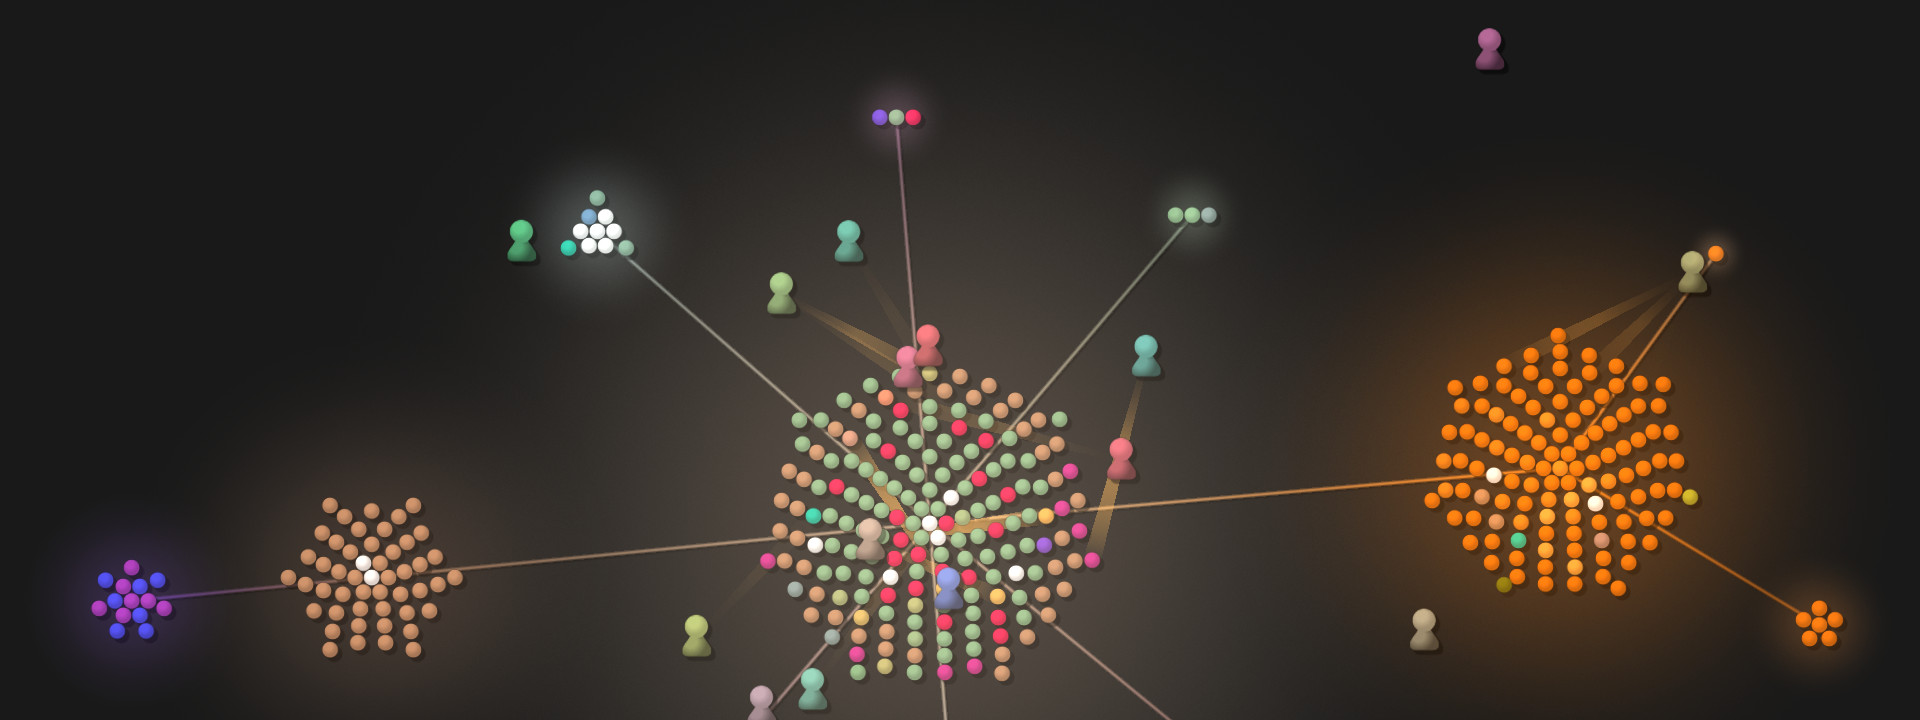
\includegraphics[scale=0.2]{Gambar/gource.jpg}
	\caption{Visualisasi proyek perangkat lunak menggunakan Gource.}
	\label{fig:gource}
\end{figure}

Gambar \ref{fig:gource} menunjukkan contoh visualisasi proyek perangkat lunak menggunakan Gource. Efek cahaya yang terdapat pada Gambar \ref{fig:gource} disebut dengan \textit{bloom}. Pada awalnya ukuran \textit{working tree} tidak terlalu besar. Setiap kali ditambahkan \textit{file} dan \textit{folder} baru, akan dibuat \textit{branch} dan \textit{leaf} baru pada \textit{working tree}.  

\ \\
Gource memiliki beberapa fitur. Fitur-fitur tersebut dapat diatur melalui \textit{command line options}. Berikut ini adalah beberapa \textit{command line options} yang terdapat pada Gource:
\begin{enumerate}
\item \texttt{gource --[WIDTH]x[HEIGHT]}\\
Opsi ini berfungsi untuk mengatur resolusi layar dari animasi. Parameter dari opsi ini adalah lebar dan panjang layar dalam satuan piksel. 

\item \texttt{gource --camera-mode [MODE]}\\
Opsi ini berfungsi untuk mengatur mode kamera pada Gource. Parameter dari opsi ini adalah mode dari kamera. Terdapat dua mode yaitu \textit{overview} dan \textit{track}. Dalam mode \textit{track}, kamera bergerak mengikuti \textit{user} yang sedang aktif. Dalam mode \textit{overview}, kamera menampilkan seluruh repositori.

\item \texttt{gource --path [PATH]}\\
Opsi untuk berfungsi untuk mengatur \textit{path} dari direktori yang akan dibuat animasinya. Opsi dari parameter ini adalah \textit{path} dari direktori.

\item \texttt{gource --start-date [YYYY-MM-DD hh:mm:ss +tz] --stop-date [YYYY-MM-DD hh:mm:ss +tz]}\\
Opsi untuk berfungsi untuk mengatur periode waktu dalam menampilkan animasi. Parameter dari opsi ini adalah waktu mulai dan waktu akhir dalam format "YYYY-MM-DD hh:mm:ss +tz". Dimana YYYY adalah tahun, MM adalah bulan, DD adalah tanggal, hh adalah jam, mm adalah menit, ss adalah detik, dan +tz adalah zona waktu. Parameter jam, menit, detik, dan zona waktu bersifat opsional.    

\item \texttt{gource --bloom-multiplier [FLOAT] }\\
Opsi untuk berfungsi untuk mengatur radius dari efek \textit{bloom}. Parameter dari opsi ini adalah radius dalam format bilangan riil.

\item \texttt{gource --bloom-intensity [FLOAT]}\\
Opsi untuk berfungsi untuk mengatur intensitas dari efek \textit{bloom}. Parameter dari opsi ini adalah intensitas \textit{bloom} dalam format bilangan riil.

\item \texttt{gource --disable-bloom}\\
Opsi ini berfungsi untuk menonaktifkan animasi \textit{bloom}.

\item \texttt{gource --date-format [FORMAT]}\\ 
Opsi untuk mengatur format waktu yang ditampilkan pada bagian tengah atas. Opsi dari parameter ini adalah format waktu dalam bentuk \textit{string}.

\item \texttt{gource --background [FFFFFF]}\\
Opsi ini berfungsi untuk mengatur warna \textit{background}. Parameter dari opsi ini adalah warna dalam format heksadesimal.

\item \texttt{gource --background-image [IMAGE]}\\
Opsi ini berfungsi untuk mengatur gambar \textit{background}. Parameter dari opsi ini adalah nama \textit{file} dari gambar.

\item \texttt{gource --font-size [SIZE]}\\
Opsi ini digunakan untuk mengatur ukuran \textit{font} pada tulisan \textit{title} dan tanggal. Parameter dari opsi ini adalah ukuran \textit{font}.  

\item \texttt{gource --font-colour [FFFFFF]}\\
Opsi ini digunakan untuk mengatur warna \textit{font} pada tulisan \textit{title} dan tanggal. Parameter dari opsi ini adalah warna \textit{font} dalam format heksadesimal.

\item \texttt{gource --logo [IMAGE]}\\
Opsi ini berfungsi untuk memasukkan logo. Parameter dari opsi ini adalah nama \textit{file} dari gambar.

\item \texttt{gource --logo-offset [X]x[Y]}\\
Opsi ini berfungsi untuk mengatur posisi dari logo. Parameter dari opsi ini adalah posisi x dan posisi y dari logo. 

\item \texttt{gource --title [TITLE]}\\
Opsi ini berfungsi untuk memberi judul. Dimana judul tersebut ditampilkan pada pojok kiri bawah layar. 

\item \texttt{gource --output-framerate [FPS]}\\
Opsi ini berfungsi untuk mengatur jumlah \textit{frame} per detik pada video animasi \textit{timelapse}. Parameter dari opsi ini adalah jumlah \textit{frame} per detik.

\item \texttt{gource --hide [DISPLAY-ELEMENT]}\\
Opsi ini berfungsi untuk menyembunyikan satu atau lebih \textit{display element}. Parameter dari opsi ini adalah elemen yang akan disembunyikan. \textit{Display element} yang dapat disembunyikan yaitu:
\begin{itemize}
\item \textit{bloom}: efek \textit{bloom}. 
\item \textit{date}: waktu.  
\item \textit{dirnames}: nama direktori. 
\item \textit{files}: ikon dari berkas. 
\item \textit{filenames}: nama berkas. 
\item \textit{root}: \textit{root directory}.
\item \textit{users}: ikon dari \textit{user}.
\item \textit{usernames}: nama dari \textit{user}.
\end{itemize}
Parameter yang berjumlah lebih dari satu dipisahkan dengan koma, contoh: \textit{bloom},\textit{root},\textit{users}.
\end{enumerate}
 
Gource dapat digunakan untuk berbagai macam proyek perangkat lunak. Program pada skripsi ini hanya akan berfokus untuk proyek perangkat lunak berbasis \textit{web}. Tidak seperti Gource yang menampilkan direktori dan \textit{file} pada animasi, program pada skripsi ini menampilkan \textit{screenshot} dari halaman utama suatu \textit{website}.      
 		
		
		\item \textbf{Melakukan analisis penggunaan Selenium WebDriver dan JGit untuk membangkitkan animasi timelapse.}\\
		{\bf Status :} Ada sejak rencana kerja skripsi.\\
		{\bf Hasil :}

		\item \textbf{Merancang perangkat lunak.}\\
		{\bf Status :} Ada sejak rencana kerja skripsi.\\
		{\bf Hasil :}

		\item \textbf{Membangun perangkat lunak.}\\
		{\bf Status :} Ada sejak rencana kerja skripsi.\\
		{\bf Hasil :}

		\item \textbf{Melakukan eksperimen dan pengujian pada perangkat lunak.}\\
		{\bf Status :} Ada sejak rencana kerja skripsi.\\
		{\bf Hasil :}

		\item \textbf{Menulis dokumen skripsi.} \\
		{\bf Status :} Ada sejak rencana kerja skripsi.\\
		{\bf Hasil :}

		
	\end{enumerate}

\section{Pencapaian Rencana Kerja}
Langkah-langkah kerja yang berhasil diselesaikan dalam Skripsi 1 ini adalah sebagai berikut:
\begin{enumerate}
\item Melakukan studi literatur tentang Selenium WebDriver, Git, dan JGit.
\item Melakukan studi literatur tentang Apache Commons CLI.
\item Melakukan analisis program sejenis.
\item Melakukan analisis penggunaan Selenium WebDriver dan JGit untuk membangkitkan animasi timelapse.
\end{enumerate}

\bibliographystyle{compj}
\bibliography{referensi} 

%\section{Kendala yang Dihadapi}
%TULISKAN BAGIAN INI JIKA DOKUMEN ANDA TIPE A ATAU C
%Kendala - kendala yang dihadapi selama mengerjakan skripsi :
%\item Terlalu banyak melakukan prokratinasi
%	\item Terlalu banyak godaan berupa hiburan (game, film, dll)
%	\item Skripsi diambil bersamaan dengan kuliah ASD karena selama 5 semester pertama kuliah tersebut sangat dihindari dan tidak diambil, dan selama 4 semester terakhir kuliah tersebut selalu mendapat nilai E
%	\item Mengalami kesulitan pada saat sudah mulai membuat program komputer karena selama ini selalu dibantu teman
%\end{itemize}

\vspace{1cm}
\centering Bandung, \tanggal\\
\vspace{2cm} \nama \\ 
\vspace{1cm}

Menyetujui, \\
\ifdefstring{\jumpemb}{2}{
\vspace{1.5cm}
\begin{centering} Menyetujui,\\ \end{centering} \vspace{0.75cm}
\begin{minipage}[b]{0.45\linewidth}
% \centering Bandung, \makebox[0.5cm]{\hrulefill}/\makebox[0.5cm]{\hrulefill}/2013 \\
\vspace{2cm} Nama: \pembA \\ Pembimbing Utama
\end{minipage} \hspace{0.5cm}
\begin{minipage}[b]{0.45\linewidth}
% \centering Bandung, \makebox[0.5cm]{\hrulefill}/\makebox[0.5cm]{\hrulefill}/2013\\
\vspace{2cm} Nama: \pemB \\ Pembimbing Pendamping
\end{minipage}
\vspace{0.5cm}
}{
% \centering Bandung, \makebox[0.5cm]{\hrulefill}/\makebox[0.5cm]{\hrulefill}/2013\\
\vspace{2cm} Nama: \pembA \\ Pembimbing Tunggal
}
\end{document}

